\documentclass[a4paper, 12pt]{article}
\usepackage[UTF8]{ctex}
% \usepackage[T1]{fontenc}
% \usepackage{inconsolata}


\usepackage{amsmath}
\usepackage{enumitem}
\setlist{
    nolistsep, % 去掉 item 和正文之间的间隔
    % labelindent=\parindent,
    leftmargin=*, % 保证小节标签缩进和上面对齐
    % labelsep=1em, % 标签后的空白
    align=left, % 标签对齐段落左边缘
}
\usepackage{tabularx}

\usepackage{graphicx}

\usepackage{geometry}
\geometry{
    a4paper,
    left=2cm,
    right=2cm,
    top=2cm,
    bottom=2cm,
}

\newcommand{\fs}[1]{\fontsize{#1 pt}{0pt}\selectfont}

\usepackage{mathtools}
\DeclarePairedDelimiter{\ceil}{\lceil}{\rceil}
\DeclarePairedDelimiter\floor{\lfloor}{\rfloor}

\usepackage{setspace}
% \setlength\parindent{0pt}
\setlength{\parindent}{2em} % 中文

% \newfontfamily\csl{Consolas}

\usepackage{array}
\newcolumntype{T}{>{\ttfamily}l}
\newcolumntype{Y}{>{\footnotesize\ttfamily}l}
\newcolumntype{y}{>{\footnotesize\ttfamily}c}

\usepackage{longtable}

\newcommand*{\thead}[1]{\multicolumn{1}{c}{\bfseries #1}}
\newcommand*{\yhead}[1]{\multicolumn{1}{c}{\footnotesize\bfseries #1}}

\newcommand{\ssa}{\phantom{x}}
\newcommand{\ssb}{\phantom{xx}}
\newcommand{\ssc}{\phantom{xxx}}
\newcommand{\ssd}{\phantom{xxxx}}
\newcommand{\sse}{\phantom{xxxxx}}

\usepackage{xcolor}
\usepackage{listings}
\definecolor{mygreen}{RGB}{28,172,0} % color values Red, Green, Blue
\definecolor{mylilas}{RGB}{170,55,241}

\newcommand{\ttf}{\ttfamily}

\lstdefinestyle{plainText}{language={},
    % basicstyle=\footnotesize \ttfamily,        % set font type and size
    basicstyle=\ttfamily,        % set font type and size
    breaklines=true,
    keywordstyle=\color{blue},
    % morekeywords={matlab2tikz},
    % morekeywords=[2]{1}, 
    % keywordstyle=[2]{\color{black}},
    identifierstyle=\color{black},
    stringstyle=\color{mylilas},
    % stringstyle=\color{purple},
    frame=single,
    framexleftmargin=0em,
    aboveskip=-\baselineskip,
    commentstyle=\color{mygreen},
    showstringspaces=false,% without this there will be a symbol in the places where there is a space
    % numbers=left,
    numbers=none,
    numberstyle={\tiny \color{black}}, % size of the numbers
    numbersep=9pt, % this defines how far the numbers are from the text
    tabsize=4,                     % sets default tabsize to 4 spaces
    emph=[1]{},
    emphstyle=[1]\color{red}, %some words to emphasise
    %emph=[2]{word1,word2}, 
    % emphstyle=[2]{style}, 
    escapeinside=``,               % Characters escape: To Use Chinese in codes   
}

\lstdefinestyle{myC}{language={C},
    % basicstyle=\footnotesize \ttfamily,        % set font type and size
    basicstyle=\ttfamily,        % set font type and size
    breaklines=true,
    keywordstyle=\color{blue},
    % morekeywords={matlab2tikz},
    % morekeywords=[2]{1}, 
    % keywordstyle=[2]{\color{black}},
    identifierstyle=\color{black},
    stringstyle=\color{mylilas},
    % stringstyle=\color{purple},
    frame=single,
    framexleftmargin=0em,
    aboveskip=-\baselineskip,
    commentstyle=\color{mygreen},
    showstringspaces=false,% without this there will be a symbol in the places where there is a space
    % numbers=left,
    numbers=left,
    numberstyle={\tiny \color{black}}, % size of the numbers
    numbersep=9pt, % this defines how far the numbers are from the text
    tabsize=4,                     % sets default tabsize to 4 spaces
    emph=[1]{printf},
    emphstyle=[1]\color{blue}, %some words to emphasise
    %emph=[2]{word1,word2}, 
    % emphstyle=[2]{style}, 
    escapeinside=``,               % Characters escape: To Use Chinese in codes   
}

\begin{document}
\begin{center}
{\fs{15}\bfseries {计算机动画原理与技术 ~作业 1 ~报告}}

\vspace{0.5\baselineskip}

{\fs{14} \kaishu 于泽汉 \hspace{1em} \textsf{No.118039910141}}
\end{center}


\textbf{\fs{15}1. 旋转动画的三种方法及其舍入误差}


\begin{itemize}[leftmargin=2em, label={}]

\item 三种方法的实现效果和对应代码见 \texttt{hw1\_rotation.html}。\\
浏览器(推荐使用 Chrome)打开可查看效果,文本编辑器打开可查看代码。\\
这里为了突出效果,在产生舍入误差的地方均只保留两位小数。


\item \textbf{方法 1}

\begin{center}
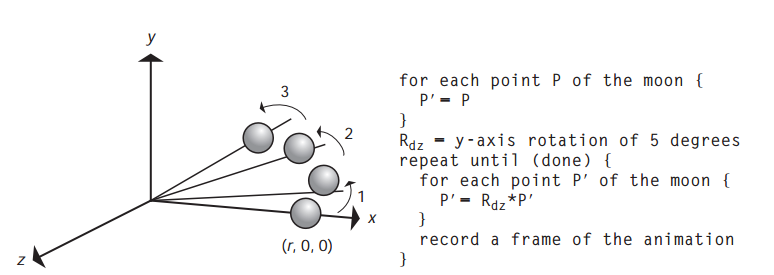
\includegraphics [width=0.8\textwidth] {./images/method_1.png}\\
\textbf{方法 1:}每次迭代,球面上的每个点坐标,乘上一个相同的旋转固定角度的矩阵
\end{center}

方法 1 的舍入误差会积累在球面上每个点的坐标数值中。

随着迭代次数的增多,这些点不再能形成标准的球面,而是会偏离应在的位置,并且原先在同一条经线或者纬线上的点之后也将不再共线。

如下各图所示:

\begin{center}
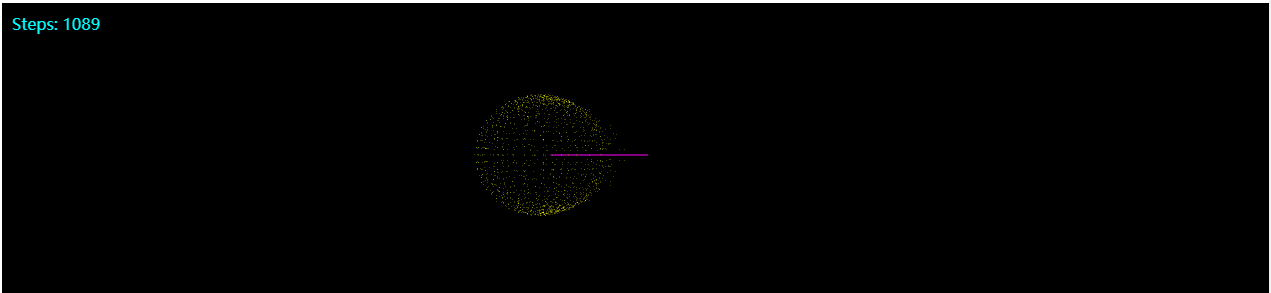
\includegraphics [width=\textwidth] {./images/step_1_1.png}\\
采用方法 1 迭代 1089 次\\[4ex]
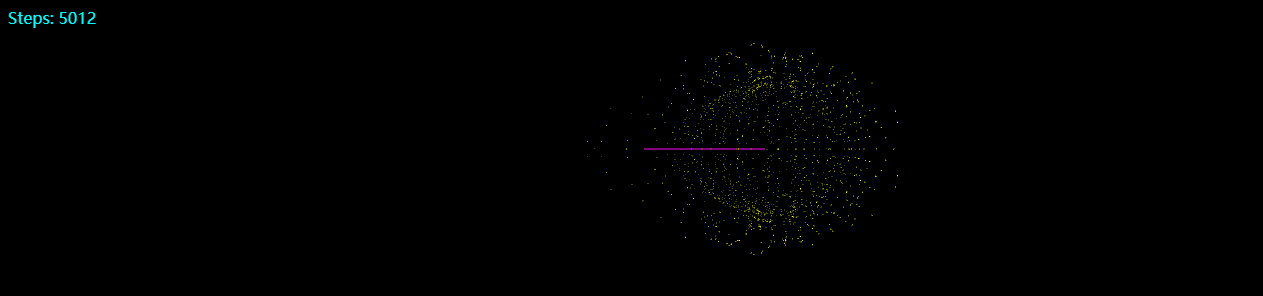
\includegraphics [width=\textwidth] {./images/step_2_1.png}\\
采用方法 1 迭代 5012 次\\[4ex]
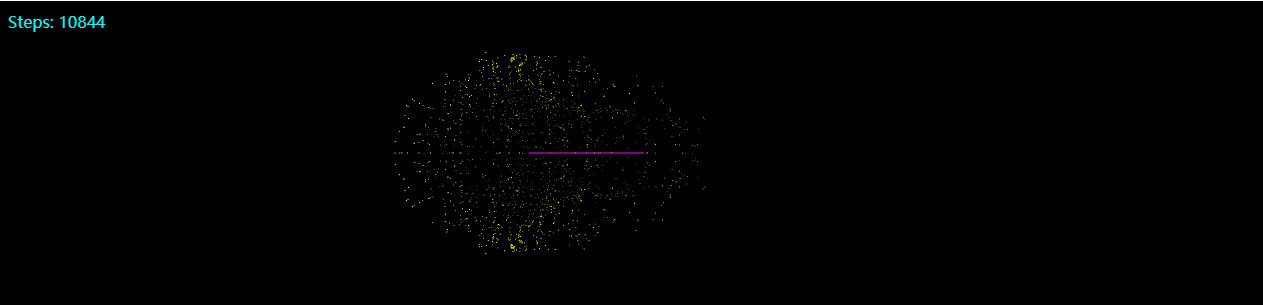
\includegraphics [width=\textwidth] {./images/step_3_1.png}\\
采用方法 1 迭代 10844 次\\[4ex]
\end{center}

迭代次数越多,偏差的程度也就越大。

\vspace{\baselineskip}

\item \textbf{方法 2}

\begin{center}
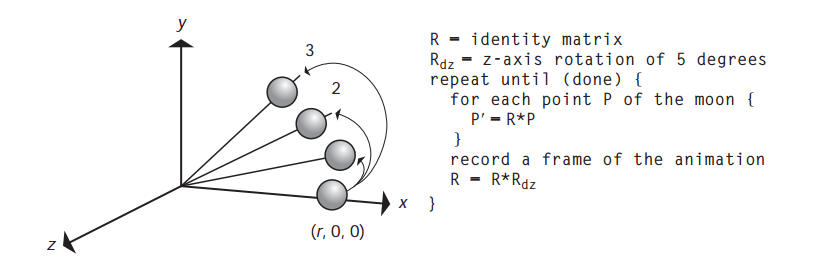
\includegraphics [width=0.8\textwidth] {./images/method_2.png}\\
\textbf{方法 2:}每次迭代,将旋转矩阵乘上一个相同的旋转固定角度的矩阵,然后再将这个旋转矩阵作用于球面上各点
\end{center}

方法 2 的舍入误差会积累在变换矩阵中。

随着迭代次数的增多,变换矩阵不再是对应的旋转矩阵,因此球面上的点可能会出现一定程度的拉伸和平移。不过原先在同一条经线或纬线上的点依旧保持共线,因为虽然该矩阵不再是单纯的旋转矩阵,但是依旧作线性变换。

如下各图所示:

\begin{center}
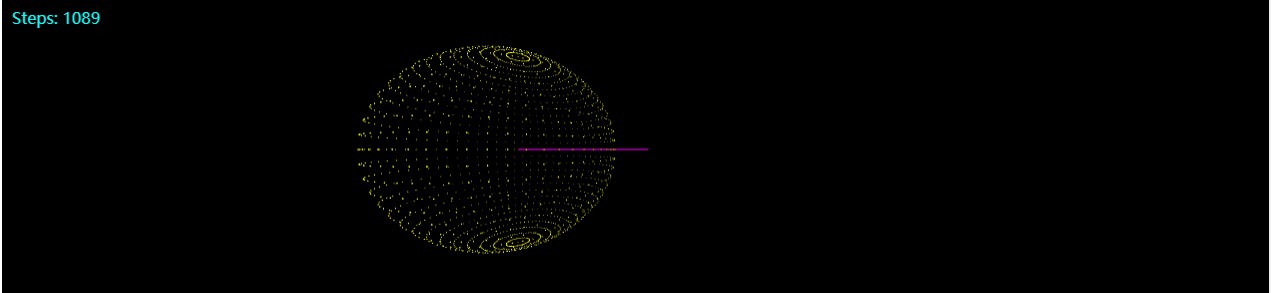
\includegraphics [width=\textwidth] {./images/step_1_2.png}\\
采用方法 2 迭代 1089 次\\[4ex]
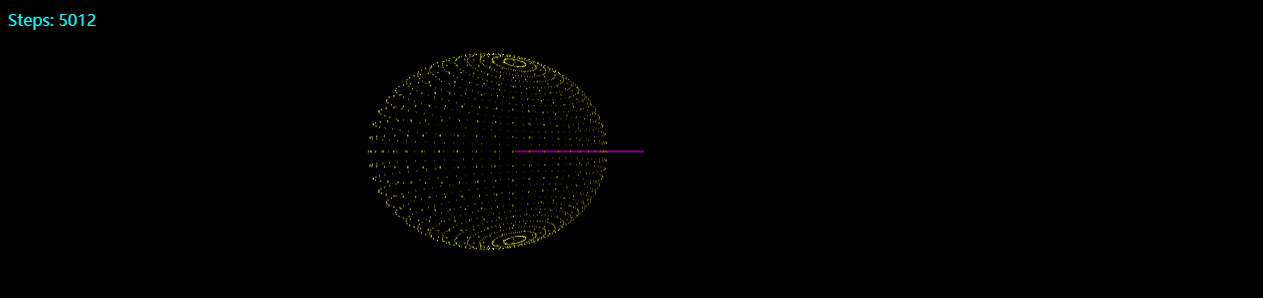
\includegraphics [width=\textwidth] {./images/step_2_2.png}\\
采用方法 2 迭代 5012 次\\[4ex]
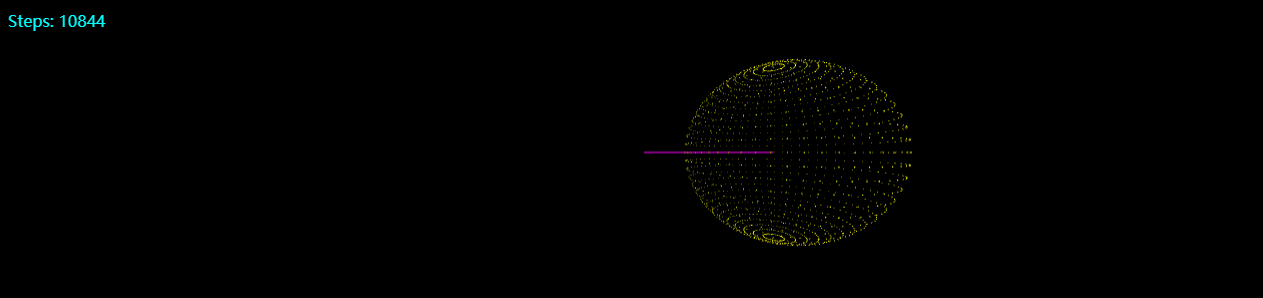
\includegraphics [width=\textwidth] {./images/step_3_2.png}\\
采用方法 2 迭代 10844 次\\[4ex]
\end{center}

随着迭代次数的增多,偏差的程度并不像方法 1 那样明显。

\vspace{\baselineskip}

\item \textbf{方法 3}

\begin{center}
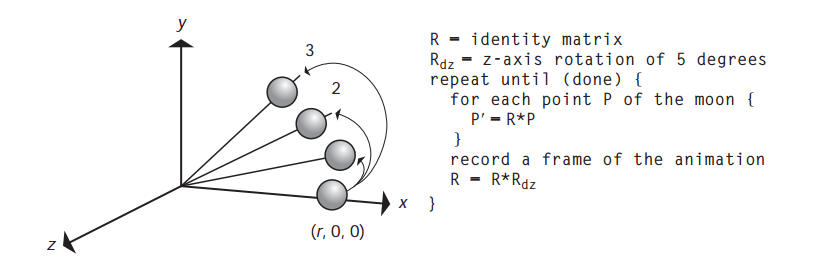
\includegraphics [width=0.8\textwidth] {./images/method_2.png}\\
\textbf{方法 3:}每次迭代,将旋转角度增加一个固定的值,再将球面上各点坐标乘上该角度对应的旋转矩阵
\end{center}

方法 3 的舍入误差会积累在旋转角度中。

随着迭代次数的增多,旋转角度出现偏差,但是依旧对应的是正常的旋转矩阵,原先在同一条经线或纬线上的点也依旧保持共线,球面上各点之间的联系没有破坏。

如下各图所示:

\begin{center}
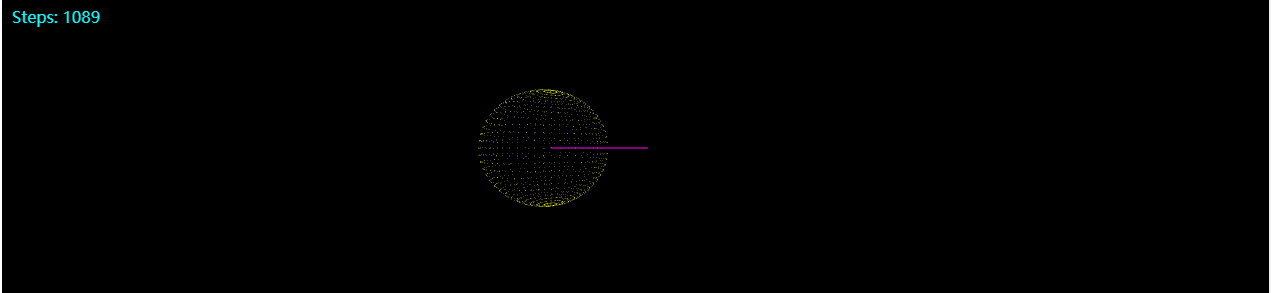
\includegraphics [width=\textwidth] {./images/step_1_3.png}\\
采用方法 3 迭代 1089 次\\[4ex]
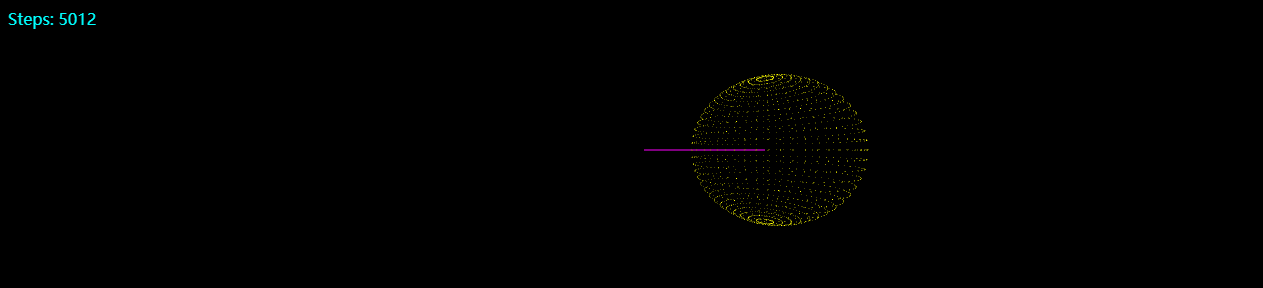
\includegraphics [width=\textwidth] {./images/step_2_3.png}\\
采用方法 3 迭代 5012 次\\[4ex]
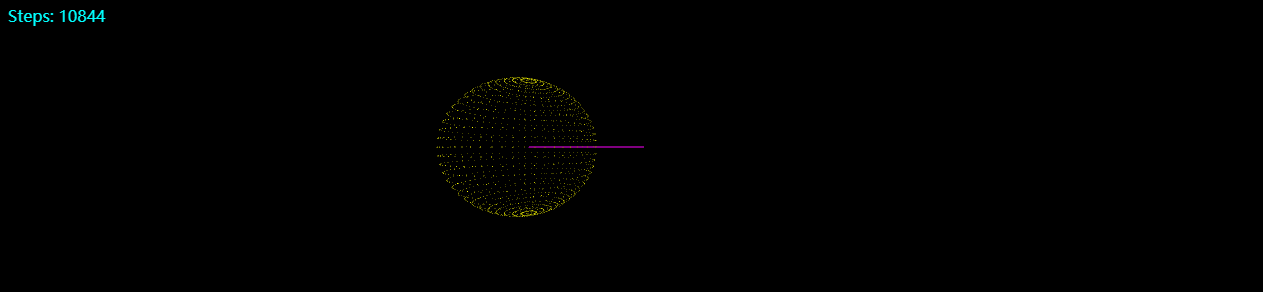
\includegraphics [width=\textwidth] {./images/step_3_3.png}\\
采用方法 3 迭代 10844 次\\[4ex]
\end{center}

随着迭代次数的增多,肉眼几乎看不出偏差(因为只有角度有误差)。


\vspace{2\baselineskip}

\item \textbf{2. 使用四元数实现旋转插值}

\item 旋转插值的实现效果和对应代码见 \texttt{hw1\_quaternion.html}。\\
浏览器(推荐使用 Chrome)打开可查看效果,文本编辑器打开可查看代码。

若两个四元数分别为 $q_1$ 和 $q_2$,那么对它们的插值(之后还要标准化)为:

$$
slerp(q_1, q_2, t) = \frac{\sin [(1-t)\theta] \cdot q_1 + \sin [t\theta]\cdot q_2}{\sin \theta}
$$

其中:$\theta$ 为 $q_1$ 和 $q_2$ 的夹角,可以通过公式计算得到;$t$ 为插值系数,取值范围为 $[0,1]$。

当然,还需要考虑很多边界情况。比如, $\theta$ 较小时需要合理近似($\sin \theta \approx \theta$)以消去接近 0 的除数;两个四元数之间角度超过 180 度时,需要对其中一个四元数取负,以使插值“不绕远路”;诸如此类,都写在代码中,这里不再赘述。



\end{itemize}

\end{document}